%versi 2 (8-10-2016)
\chapter{Landasan Teori}
\label{chap:teori}
Bab ini menjelaskan dasar teori mengenai {\it Wireless Sensor Network}, {\it Accelerometer} , {\it Feature Extraction}, {\it Fourier Transform}, dan Preon32 

\section{Wireless Sensor Network}
\label{sec:wirelesssensornetwork} 
{\it Wireless Sensor Network} (WSN) adalah jaringan nirkabel berupa kumpulan dari {\it node} sensor yang dapat saling berkomunikasi, melakukan komputasi, dan melakukan pengukuran pada lingkungan {\it node} tersebut diletakkan. \cite{fundamentals:0:fundamental} Pengukuran yang dapat dilakukan seperti getaran, suhu, kelembapan udara, suara, dan lainnya. Setiap data hasil pengukuran atau {\it sensing} pada {\it node} dikirimkan ke {\it base station} untuk diproses. 

\subsection{Aplikasi dari Wireless Sensor Network \cite{kazem:0:wsn}}
\label{subsec:aplikasiWSN}
WSN secara umum digunakan pada {\it high-end application} dan daerah - daerah yang tidak dapat dicakup oleh {\it wiredline system} seperti sistem pendeteksi radiasi dan {\it nuclear-threat}. Semakin lama WSN terus dikembangkan dan juga diaplikasikan pada bidang sebagai berikut:
\begin{itemize}
	\item Aplikasi bidang Militer : pemantauan serangan musuh, mendeteksi serangan nuklir/biologis/kimia, penargetan , dan lainya (Gambar~\ref{fig:militaryApplicationExample}).
		\begin{figure} [H]
			\centering  
			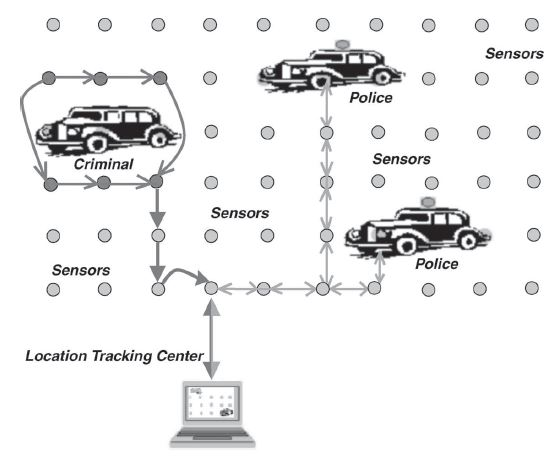
\includegraphics[scale=0.7]{militaryApplicationExample}  
			\caption[Contoh aplikasi WSN pada bidang militer]{Contoh aplikasi WSN pada bidang militer} 
			\label{fig:militaryApplicationExample} 
		\end{figure} 	
	\item Aplikasi bidang Lingkungan/area : pendeteksi kebakaran hutan, pendeteksi kebanjiran, {\it microclimate}(kondisi iklim daerah yang kecil), dan lainya.
	\item Aplikasi bidang Kesehatan : pelacakkan dan pemantauan pasien dan doktor dalam rumah sakit, pemantauan pemberian obat, membantu pasien disabilitas, dan lainnya.
	\item Aplikasi bidang Industri	: pendeteksi asap, pemantauan peralatan, pemantauan keamanan, automasi, dan lainnya.
\end{itemize}

Secara mendasar WSN dapat diaplikasikan saat dibutuhkan alat pemantauan yang dapat bereaksi dengan lingkungan tertentu.

\subsection{Sensor Node \cite{holger:0:protchitect}}
\label{subsec:sensorNode} 
Struktur pada sensor node memiliki 5 komponen utama, yaitu {\it power supply}, {\it controller}, {\it memory}, {\it sensor / actuator}, dan {\it communication device}  (Gambar~\ref{fig:sensor_node}).

\begin{figure} [H]
	\centering  
	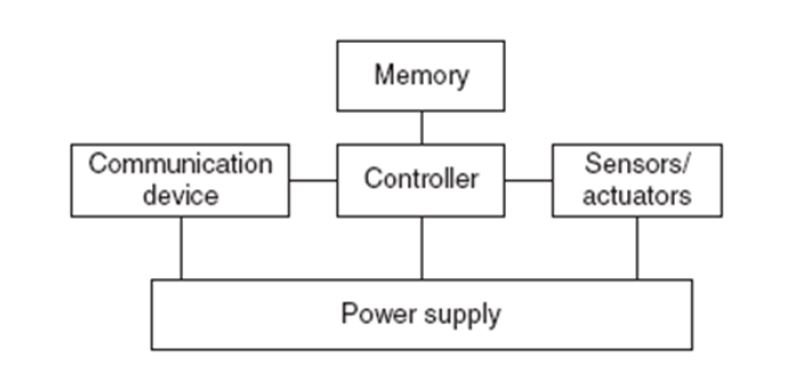
\includegraphics[scale=0.8]{sensor_node}  
	\caption[Struktur Sensor Node]{Struktur Sensor Node} 
	\label{fig:sensor_node} 
\end{figure} 

\subsubsection{Power Supply}
{\it Power supply} berfungsi sebagai sumber energi untuk sensor node. Secara umum {\it power supply} yang digunakan oleh sensor node berupa baterai.

\subsubsection{Controller}
{\it Controller} merupakan inti dari sensor node. {\it Controller} berfungsi untuk mengumpulkan data dari sensor, menerima data dari sensor node lain, memroses data, menentukan tujuan data dikirim, dan menentukan waktu data dikirim. Di dalam {\it controller} terdapat {\it microcontroller / microprocessor} yang berfungsi untuk mengatur data dan melakukan komputasi. Beberapa contoh dari {\it microcontroller} sebagai berikut : 
	\begin{enumerate}
		\item Intel StrongARM
		\item Texas Instruments MSP 430
		\item Atmel ATmega
	\end{enumerate}
			
\subsubsection{Memory}
{\it Memory} pada sensor node adalah berupa {\it Random Access Memory} (RAM). {\it Memory} bersifat {\it volatile}, yaitu jika sensor node mati maka tidak ada data yang disimpan pada  sensor node dan setiap data yang disimpan pada {\it memory} akan hilang.

\subsubsection{Sensor / Actuator}
{\it Sensor} pada sensor node berfungsi sebagai antarmuka langsung terhadap lingkungan dan {\it Actuator} berfungsi sebagai pengubah sinyal dari lingkungan menjadi aksi fisik. Contoh dari {\it actuator} adalah LED yang dapat mengubah listrik menjadi cahaya. Ada beberapa tipe dari sensor:
\begin{itemize}
	\item {\it Passive, omnidirectional sensors} : Sensor ini dapat mengukur lingkungan tanpa harus memanipulasi lingkungan dan tidak terpengaruh dari arah sensor tersebut diletakkan. Beberapa contohnya adalah {\it thermometer}, {\it light sensor}, {\it vibration / accelerometer}, {\it microphones}, {\it humidity}, {\it smoke detectors}, {\it air pressure}, dan lainnya.
	\item {\it Passive, narrow-beam sensors} : Sensor ini  dapat mengukur lingkungan tanpa harus memanipulasi lingkungan, tetapi berpengaruh terhadap arah sensor tersebut diletakkan. Salah satu contohnya adalah kamera yang dapat langsung mengukur jarak.
	\item {\it Active sensors} : Sensor ini mengukur lingkungan dengan terus menerus memeriksa lingkungan. Sebagai contoh {\it radar}, {\it sonar}, atau {\it seismic sensor} yang memancarkan gelombang - gelombang untuk melakukan pengukuran.
\end{itemize}

\subsubsection{Communication Device}
{\it Communication device} berfungsi sebagai alat untuk mengirim dan menerima informasi dari sensor node lain. Ada beberapa tipe / jalur dari komunikasi pada sensor node (Gambar~\ref{fig:singleHopvsmultiHop}) , yaitu:
\begin{itemize}
	\item {\it Single Hop} : Komunikasi ini adalah komunikasi langusng antara sensor node dengan {\it base station} / {\it sink}, sehingga seperti satu loncatan / {\it hop}.
	\item {\it Multi Hop} : Komunikasi ini memerlukan sensor node lain sebagai loncatan / {\it hop} untuk berkomunikasi dengan {\it base station} / {\it sink}. Jika sensor node ingin mengirimkan informasi ke {\it base station} maka sensor node mengirimkan informasi tersebut ke sensor node terdekat dan terus sampai ke {\it base station}.
\end{itemize}

\begin{figure} [H]
	\centering  
	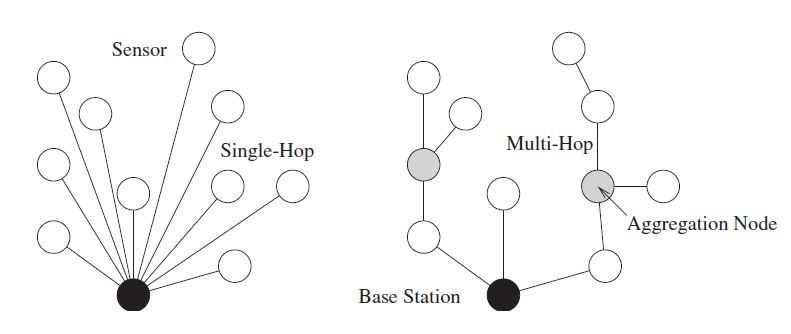
\includegraphics[scale=0.8]{singleHopvsmultiHop}  
	\caption[{\it Single Hop} dan {\it Multi Hop}]{{\it Single Hop} dan {\it Multi Hop}} 
	\label{fig:singleHopvsmultiHop} 
\end{figure} 

\subsection{Topologi pada WSN \cite{topologi:0:topologiWSN}}
\label{subsec:topologiWSN}
WSN umumnya memiliki banyak sensor node yang diletakkan pada suatu tempat. Pada WSN bisa terdapat satu atau lebih {\it sink} atau {\it base station}. {\it sink} adalah sensor node yang bertugas untuk mendapatkan data dari sensor node lain. Jalur dan cara komunikasi sensor node dengan sensor node lain / {\it sink} bergantung pada topologi WSN yang digunakan.

\subsubsection{Bus Topology}
Pada {\it Bus Topology} (Gambar~\ref{fig:bus}), semua node terhubung pada satu jalur untuk saling berkomunikasi.Jika sensor node mengirim pesan maka sensor node akan mengirim pesan secara bergantian dan mengirim {\it broadcast message} ke semua sensor node, tetapi hanya sensor node yang dituju akan menerima dan memroses message tersebut. Kelebihan dari topologi bus ini adalah mudah untuk diimplementasi ,tetapi kelemahannya adalah satu jalur tunggal untuk berkomunikasi yang jika jalur tersebut bermasalah maka sensor node tidak dapat berkomunikasi.
\begin{figure} [H]
	\centering  
	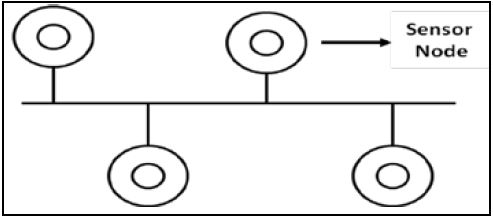
\includegraphics[scale=0.8]{bus}  
	\caption[{\it Bus Topology}]{{\it Bus Topology}} 
	\label{fig:bus} 
\end{figure} 

\subsubsection{Tree Topology}
\label{subsubsec:treeTop}
Pada {\it Tree Topology} (Gambar~\ref{fig:tree}), sensor node disusun secara hierarki dan terdapat sensor node yang disebut {\it root node} pada level teratas. {\it Root node} bertugas sebagai {\it communication router} utama / sebagai {\it base station}. Selain {\it root node} terdapat sensor node yang disebut {\it children node} dan {\it parent node}. {\it Children} dari sensor node adalah sensor node yang memiliki level lebih rendah dari sensor node tersebut dan {\it parent} dari sensor node adalah sensor node yang memiliki level lebih tinggi dari sensor node tersebut.  Saat sensor node mengirim pesan, sensor node akan meneruskan pesan dari {\it children} dari sensor node tersebut  ke {\it parent} dari sensor node tersebut hingga sampai ke {\it base station}.  Kelebihan dari topologi ini adalah jika terjadi kesalahan pada sensor node maka akan mudah diidentifikasi dengan cara menelusuri {\it children} dari sensor node tersebut, tetapi kelemahan dari topologi ini adalah sulit untuk dikonfigurasi dan jika ada jalur yang putus di salah satu sensor node maka akan memutuskan semua komunikasi bagi {\it children} dari sensor node tersebut.
\begin{figure} [H]
	\centering  
	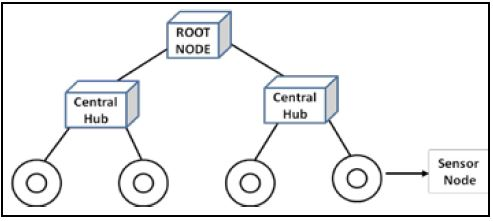
\includegraphics[scale=0.8]{tree}  
	\caption[{\it Tree Topology}]{{\it Tree Topology}} 
	\label{fig:tree} 
\end{figure} 

\subsubsection{Star Topology}
\label{subsubsec:starTop}
Pada {\it Star Topology} (Gambar~\ref{fig:star}), semua node terhubung dengan {\it centralized communication hub (sink)} dan sensor node tidak dapat secara langsung berkomunikasi dengan sensor node lainnya. Jika sensor node ingin mengirim pesan ke sensor node lain, maka sensor node harus mengirim pesan ke {\it sink} lalu {\it sink} meneruskan pesan tersebut ke sensor node yang dituju. Jika {\it sink} terjadi kerusakkan, maka sensor node tidak dapat berkomunikasi dan jaringan tersebut mati.
\begin{figure} [H]
	\centering  
	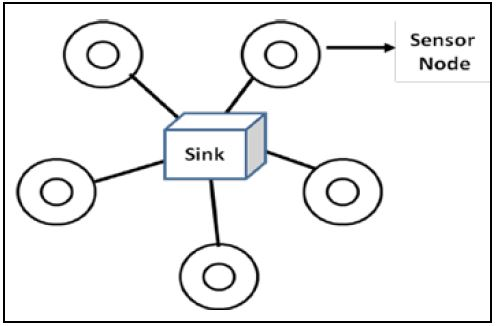
\includegraphics[scale=0.8]{star}  
	\caption[{\it Star Topology}]{{\it Star Topology}} 
	\label{fig:star} 
\end{figure} 

\subsubsection{Ring Topology}
Pada {\it Ring Topology} (Gambar~\ref{fig:ring}), semua node pasti memiliki dua node tetangga dan dihubungkan secara melingkar. Jika sensor node mengirim pesan,  maka pesan tersebut akan diteruskan ke sensor node lain secara melingkar hingga sampai ke sensor node yang dituju. Kelebihan dari sensor node ini adalah mudah untuk diimplementasikan, tetapi jika ada sensor node yang rusak dan membuat kegagalan dalam mengirim pesan, maka sensor node akan mengirimkan kembali pesan ke arah melingkar yang sebaliknya.
\begin{figure} [H]
	\centering  
	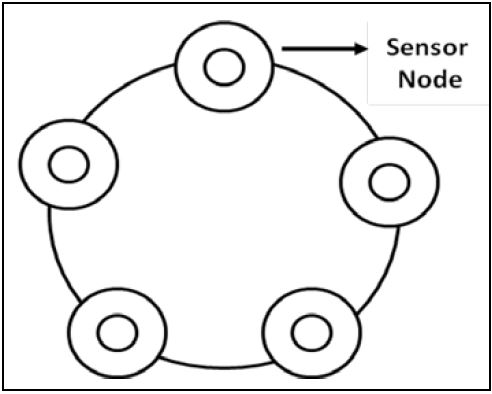
\includegraphics[scale=0.8]{ring}  
	\caption[{\it Ring Topology}]{{\it Ring Topology}} 
	\label{fig:ring} 
\end{figure} 

\subsubsection{Mesh Topology}
Terdapat 2 tipe dari topologi mesh yaitu, {\it full mesh} dan {\it partial mesh} (Gambar~\ref{fig:mesh}). Jika semua sensor node saling terhubung satu sama lain, maka itu adalah {\it full mesh}. Jika ada sensor node terhubung secara tidak langsung dengan sensor node lain, maka itu adalah {\it partial mesh}.
\begin{figure} [H]
	\centering  
	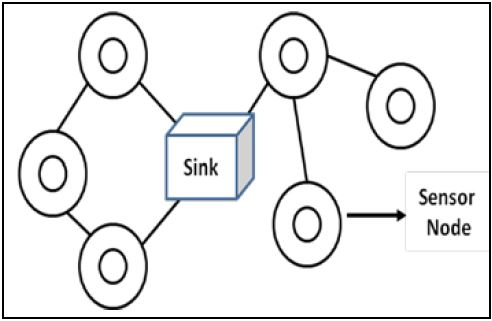
\includegraphics[scale=0.8]{mesh}  
	\caption[{\it Mesh Topology}]{{\it Mesh Topology}} 
	\label{fig:mesh} 
\end{figure} 

\subsubsection{Circulation Topology}
(Gambar~\ref{fig:circular}) Topologi ini disebut juga dengan topologi {\it circular web} karena sensor node diletakkan seperti membentuk jaring yang melingkar dan {\it sink} sebagai pusat dari jaring. Kelebihan dari topologi ini adalah mudah untuk dibangun, dirawat, dan lebih efisien secara energi \cite{topologi:0:topologiWSN}.
\begin{figure} [H]
	\centering  
	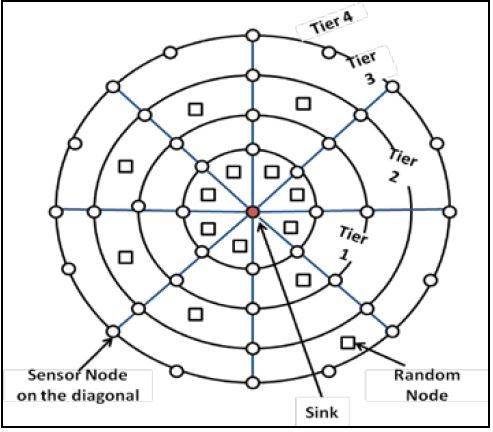
\includegraphics[scale=0.8]{circular}  
	\caption[{\it Circular Topology}]{{\it Circular Topology}} 
	\label{fig:circular} 
\end{figure} 

\subsubsection{Grid Topology}
Pada {\it Grid Topology} (Gambar~\ref{fig:grid}), area dari jaringan dipartisi secara merata menjadi {\it grid - grid} dan seluruh sensor node dibagi - bagi sesuai {\it grid}. Pada setiap {\it grid}, sensor node harus aktif secara bergantian sehingga terdapat satu sensor node yang aktif dalam satu {\it grid} walaupun dalam {\it grid} tersebut terdapat lebih dari satu sensor node. Sensor node yang aktif bertugas mengirim atau meneruskan informasi ke sensor node lain sesuai dengan hasil rute dari {\it Grid-based multi-path routing protocol} hingga sampai ke {\it sink}.
\begin{figure} [H]
	\centering  
	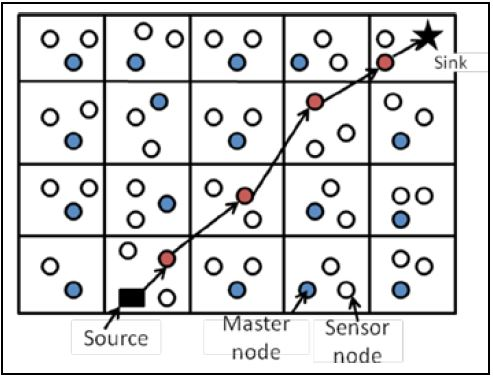
\includegraphics[scale=0.8]{grid}  
	\caption[{\it Grid Topology}]{{\it Grid Topology}} 
	\label{fig:grid} 
\end{figure} 

\subsection{Arsitektur WSN \cite{jun:0:wsnpers}}
\label{subsec:arch}
WSN dapat dibuat dengan arsitektur {\it flat} atau {\it hierarchy}. Arsitektur pada WSN mempengaruhi tugas - tugas pada setiap sensor node pada WSN. 

\subsubsection{Flat Architecture}
\label{subsubsec:flatArch}
Seluruh sensor node pada aritektur ini (Gambar~\ref{fig:flatArchitecture}) memiliki tugas yang sama dalam {\it sensing} dan setiap sensor node merupakan {\it peers}. Jika {\it sink} ingin mengumpulkan data maka {\it sink} akan mengirim {\it query} dengan teknik {\it flooding} ke seluruh sensor node dan hanya sensor node yang cocok dengan query tersebut akan merespon kembali ke {\it sink}. Seluruh sensor node melakukan komunikasi {\it multi hop} dengan menggunakan sensor node lain sebagai penyampai data untuk berkomunikasi dengan {\it sink}.
\begin{figure} [H]
	\centering  
	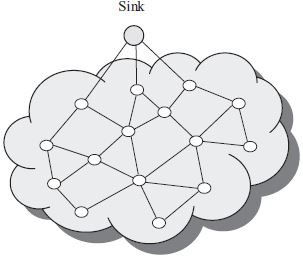
\includegraphics[scale=1]{flatArchitecture}  
	\caption[{\it Flat Architecture}]{{\it Flat Architecture}} 
	\label{fig:flatArchitecture} 
\end{figure} 

\subsubsection{Hierarchy Architecture}
\label{subsubsec:hierarchyArch}
Arsitektur ini mengelompokkan seluruh sensor node menjadi {\it cluster - cluster}. Dalam {\it cluster} terdapat {\it cluster head} dan {\it cluster member}. {\it Cluster head} bertugas untuk menerima data dari {\it cluster member} dan mengirimkan data tersebut ke {\it sink}. {\it Cluster} member bertugas untuk mengirimkan data hasil pengukuran ke {\it cluster head}. Dalam {\it cluster}, sensor node yang memiliki energi yang terbesar dapat dipilih menjadi {\it cluster head} dan yang lainnya akan menjadi {\it cluster member}. Selain itu {\it cluster head} dapat dipilih berdasarkan jarak {\it cluster head} ke {\it cluster member}, {\it single hop} (Gambar~\ref{fig:singleHopArchitecture})/{\it multi hop} (Gambar~\ref{fig:multihopclusteringarchitecture}), dan berdasarkan jumlah {\it tier} (Gambar~\ref{fig:multitierClusteringarchitecture}).
\begin{figure} [H]
	\centering  
	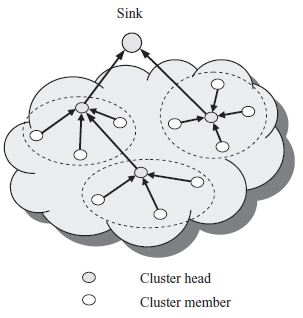
\includegraphics[scale=1]{singleHopArchitecture}  
	\caption[{\it Single Hop Architecture}]{{\it Single Hop Architecture}} 
	\label{fig:singleHopArchitecture} 
\end{figure} 
\begin{figure} [H]
	\centering  
	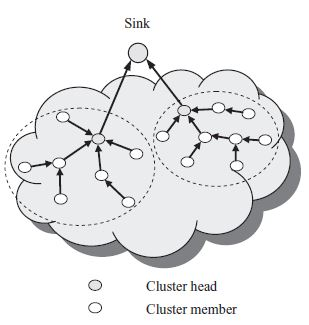
\includegraphics[scale=1]{multihopclusteringarchitecture}  
	\caption[{\it Multi Hop Clustering Architecture}]{{\it Multi Hop Clustering Architecture}} 
	\label{fig:multihopclusteringarchitecture} 
\end{figure} 
\begin{figure} [H]
	\centering  
	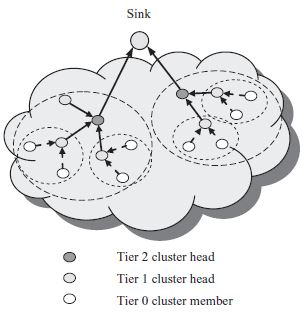
\includegraphics[scale=1]{multitierClusteringarchitecture}  
	\caption[{\it Multi Tier Clustering Architecture}]{{\it Multi Tier Clustering Architecture}} 
	\label{fig:multitierClusteringarchitecture} 
\end{figure} 

\subsection{Sistem Operasi WSN \cite{fundamentals:0:fundamental}}
Setiap sensor node pada WSN membutuhkan sistem operasi untuk mengatur berjalannya sensor node. Sistem operasi bertugas untuk aplikasi bisa berkomunikasi dengan {\it hardware}, {\it scheduling tasks} dan {\it prioritize tasks}, {\it memory management}, {\it power management}, {\it file management}, dan lainnya. Berikut contoh sistem operasi dari WSN: 
\begin{itemize}
	\item TinyOS
	\item Contiki
	\item MANTIS
	\item Nano-RK
	\item LiteOS
	\item PreonVM
\end{itemize}  

\subsection{Protokol Stack WSN \cite{jun:0:wsnpers}}
\begin{figure} [H]
	\centering  
	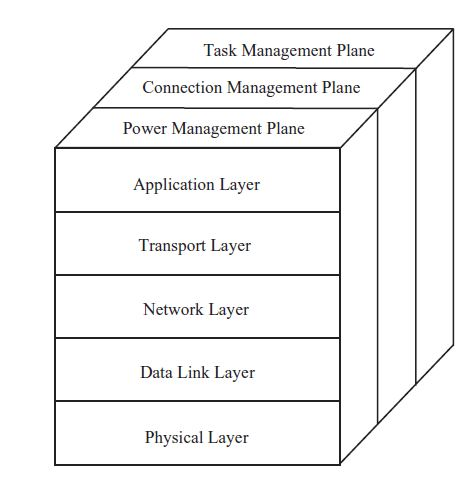
\includegraphics[scale=1]{protocolStack}  
	\caption[Protokol Stack WSN]{Protokol Stack WSN} 
	\label{fig:protocolStack} 
\end{figure} 

Protocol Stack pada WSN terdiri dari tiga management (Gambar~\ref{fig:protocolStack}), yaitu
\begin{itemize}
\item {\it Power Management Plane} : {\it Power management plane} berkewajiban untuk mengatur power level dari sensor node untuk sensing, processing, dan transmission dan reception. Sebagai contoh sensor node dapat mematikan transceiver saat tidak ada data yang akan dikirim atau diterima. 
\item {\it Connection Management Plane} : {\it Connection management plane} berkewajiban untuk {\it configuration / reconfiguration} koneksi sensor node saat adanya perubahan topologi pada wsn seperti penambahan atau pengurangan sensor node, perubahan letak node, dan lainnya.
\item {\it Task Management Plane} : {\it Task management plane} berkewajiban dalam medistribusikan tugas (task) pada sensor node agar meningkatkan efisiensi energi pada WSN.
\end{itemize}  
Ketiga manajemen tersebut terdapat pada 5 layer protokol stack ,yaitu
\begin{enumerate}
	\item {\it Application Layer} : 
	Pada {\it Application Layer} terdapat bermacam - macam {\it application-layer protocol} untuk {\it sensor network application} seperti {\it query dissemination}, {\it node localization}, {\it time synchronization}, dan {\it network security}. Sebagai contoh, {\it Sensor Management Protocol} (SMP) adalah {\it application-layer management protocol} yang menyediakan operasi perangkat lunak untuk berbagai {\it task}, seperti {\it exchanging location - related data}, {\it synchronization sensor nodes}, {\it moving  sensor nodes}, {\it scheduling sensor nodes}, dan {\it querying the status of sensor nodes}. 
	\item {\it Transport Layer} : 
	{\it Transport Layer} berkewajiban dalam {\it reliable end - to - end data delivery} untuk sensor ke sensor atau sensor ke {\it sink}. Terdapat 2 cara pengiriman yaitu {\it upstream} dan {\it downstream}. {\it Upstream} berarti sensor node mengirimkan data ke {\it sink}. {\it Downstream} berarti {\it sink} mengirimkan data ke sensor node. Kebutuhan {\it reliabilty} dari {\it upstream} dan {\it downstream} berbeda. {\it Downstream} membutuhkan {\it reliable delivery} karena {\it sink} hanya mengirimkan data ke sensor node satu kali. {\it Upstream} tidak terlalu membutuhkan {\it reliable delivery} karena sensor node mengirimkan data hasil {\it sense} ke {\it sink} secara terus menerus sehingga dapat terjadi pengulangan.
	\item {\it Network Layer} : 
	{\it Network Layer} bertugas dalam membuat rute komunikasi dari sensor node ke {\it sink}. {\it Network Layer} menentukan {\it single hop} / {\it multi hop} komunikasi untuk sensor node agar optimal.
	\item {\it Data Link Layer} : 
	{\it Data Link Layer} berkewajiban dalam {\it data stream multiplexing}, {\it data frame creation and detection}, {\it medium access}, dan {\it error control} untuk {\it reliable point - to - point} dan {\it point - to - multipoint transmissions}. Salah satu fungsi terpenting dari data link layer adalah {\it medium access control} (MAC). Objektif utama dari MAC adalah agar sensor node - sensor node dapat secara adil dan efisien berkomunikasi untuk perfomansi dalam konsumsi energi, {\it network throughput}, dan {\it delivery latency}.
	\item {\it Physical Layer}
	{\it Physical Layer} berkewajiban dalam mengonversi {\it bit stream} dari {\it data link layer} menjadi sinyal yang cocok untuk ditransimisi pada media komunikasi.
\end{enumerate}

\section{Akselerometer \cite{pavel:0:sensor}}
\label{sec:aks}
Salah satu sensor yang ada pada {\it node} sensor adalah sensor akselerometer. Secara umum akselerometer adalah alat yang mengukur {\it linear (not angular) acceleration}. {\it Accelerometer} memiliki kemampuan untuk mengukur akselerasi, kemiringan, dan getaran statis (gravitasi bumi) atau dinamis pada 1 sumbu $x$/$y$/$z$ ({\it single axis}) atau 2 sumbu ($x$,$y$)/($x$,$z$)/($y$,$z$) ({\it two axis}) atau 3 sumbu ($x$,$y$,$z$) ({\it three axis}). 

Akselerometer dapat dibagi menjadi 2 jenis yaitu :
	\begin{itemize}
		\item {\it Absolute accelerometer} : Akeselerometer ini terpasang langsung pada objek yang diukur.
		\item {\it Relative accelerometer} : Akeselerometer ini mengukur jarak antara objek yang diukur dan {\it reference point} yang stabil atau bergerak secara konstan. Akselerasi baru didapatkan dengan melakukan diferensiansi ganda pada jarak. Akeselerometer ini sering digunakan untuk mengukur getaran dari jarak tertentu (contoh: {\it laser vibrometer}).
	\end{itemize}
{\it Acceleration sensor} dapat diklasifikasi berdasarkan {\it physical principle} yang digunakan yaitu:
	\begin{itemize}
		\item {\it Direct Measurement of Force} : pengukuran secara langsung pada gaya, sebagai contoh {\it piezoelectric sensor}. 
		\item {\it Indirect Measurement} : pengukuran berdasarkan  perpindahan atau deformasi dari {\it sensing element}.
	\end{itemize}


\section{Feature Extraction \cite{isabelle:0:extractionFeature}}
\label{sec:fE}
Ekstraksi fitur dibagi menjadi 2 proses, yaitu 
\begin{itemize}
	\item {\it Feature Construction} : {\it Feature} sama dengan {\it input variable} / atribut. Proses {\it feature constraction} disebut juga dengan {\it preprocessing}. Ada berbagai macam {\it preprocessing}, yaitu :
	\begin{itemize}
		\item {\it Standardization} : menyamakan satuan input, sebagai contoh jika panjang diukur dalam meter dan lebar diukur dalam centimeter maka perlu disamakan satuannya antara meter atau centimeter.
		\item {\it Normalization} : data dari input dinormalisasi dengan teknik normalisasi tertentu bergantung dengan tipe datanya.
		\item {\it Signal enhancement} : input berupa sinyal dapat ditingkatkan dengan melakukan {\it signal filter}.
		\item {\it Extraction of local features} : melakukan {\it encode} pada pengetahuan yang spesifik pada suatu masalah menjadi {\it feature}.
		\item {\it Linear and non-linear space embedding methods} : Jika dimensi dari data sangat besar, maka data tersebut butuh diperkecil menjadi dimensi yang lebih kecil dan mempertahankan informasi yang terkandung pada data tersebut.
		\item {\it Non-linear expansions} : melakukan pembesaran dimensi dari data.
		\item {\it Feature discretization} : beberapa algoritma tidak dapat menangani data yang kontiniu sehingga data perlu didiskritkan.
	\end{itemize}
	\item {\it Feature Selection} : proses untuk memilih fitur yang paling informatif dan relevan. Tujuan dari proses ini adalah :
	\begin{itemize}
		\item {\it general data reduction} : membatasi penyimpanan dan mempercepat algoritma.
		\item {\it feature set reduction} : menyimpan {\it resources} pada saat pemanfaatan.
		\item {\it performance improvement} : meningkatkan perfomansi dan mendapatkan akurasi prediksi yang lebih baik.
		\item {\it data understanding} : mendapatkan pengetahuan dalam proses yang membuat data tersebut atau dengan mevisualisasi data tersebut.
	\end{itemize}
\end{itemize}

\section{Fourier Transform \cite{steven:0:dsp}} 
\label{sec:fourier}
{\it Fourier Transform} merupakan teknik matematika yang secara mendasar menguraikan sinyal menjadi {\it sinusoids}. Sinyal yang diuraikan dapat berupa sinyal {\it continuous} atau sinyal {\it discrete} dan {\it periodic} atau {\it aperiodic}. Sinyal {\it periodic} berarti sinyal tersebut akan memiliki pola yang berulang dan sinyal {\it aperiodic} berarti sinyal tersebut tidak memiliki pola yang berulang. {\it Fourier Transform} dibagi menjadi 4 kategori (Gambar~\ref{fig:signalAP}) berdasarkan jenis dari sinyal yaitu:
\begin{itemize}
	\item {\it Aperiodic-Continuous} : {\it Fourier Transform} dengan tipe sinyal ini disebut {\it Fourier Transform}.
	\item {\it Periodic-Continuous} : {\it Fourier Transform} dengan tipe sinyal ini disebut {\it Fourier Series}.
	\item {\it Aperiodic-Discrete} : {\it Fourier Transform} dengan tipe sinyal ini disebut {\it Discrete Time Fourier Transform}.
	\item {\it Periodic-Discrete} : {\it Fourier Transform} dengan tipe sinyal ini disebut {\it Discrete Fourier Transform / Discrete Fourier Series}.
\end{itemize}  

\begin{figure} [H]
	\centering  
	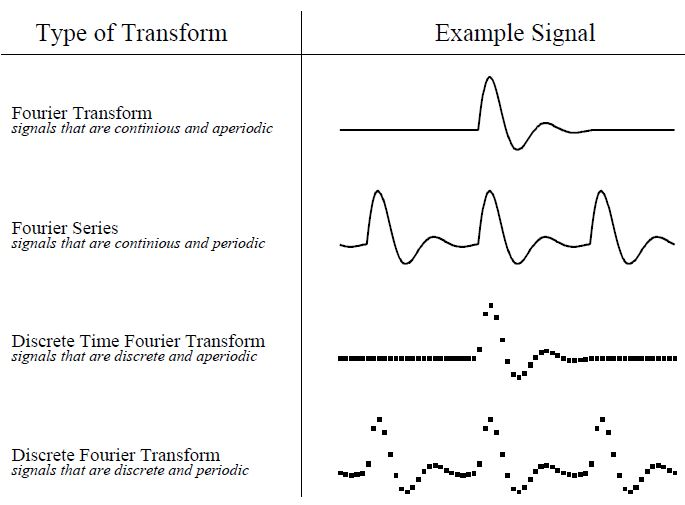
\includegraphics[scale=1]{signalAP}  
	\caption[4 kategori dari {\it Fourier Transform} dan contoh bentuk sinyal]{4 kategori dari {\it Fourier Transform} dan contoh bentuk sinyal} 
	\label{fig:signalAP} 
\end{figure} 

Keempat kategori {\it fourier transform} memiliki dua versi yaitu {\it real version} dan {\it complex version}. {\it Real version} menggunakan bilangan {\it real} dan {\it complex version} menggunakan bilangan kompleks ({\it complex number}). Pada perkembangannya penggunaan bilangan kompleks lebih banyak digunakan karena bilangan kompleks mengurangi persamaan yang digunakan. Sebagai contoh algoritma {\it Fast Fourier Transform} berdasarkan bilangan kompleks dalam perhitungannya.   

\subsection{Complex Number \cite{steven:0:dsp}}
\label{subsec:complex}

{\it Complex number} adalah penjumlahan dari dua komponen yaitu komponen {\it real} (variabel $a$ pada persamaan \ref{eqn:complexNumber}) dan komponen {\it imaginary} (variabel $b$ pada persamaan \ref{eqn:complexNumber}). Komponen {\it real} adalah {\it real number} . Komponen {\it imaginary} adalah bilangan imajiner (persamaan \ref{eqn:imNumber}).

	\begin{equation}\label{eqn:complexNumber}
		a + bj 
	\end{equation}  
	\begin{equation}\label{eqn:imNumber}
		j = \sqrt{-1}
	\end{equation}

Operasi tambah, kurang, kali, dan bagi untuk {\it complex number} memiliki aturan sebagai berikut:
\begin{itemize}
	\item operasi tambah
		\begin{equation}\label{eqn:complexNumberTambah}
			(a + bj) + (c + dj) = (a + c) + j(b + d)
		\end{equation}  
	\item operasi kurang
		\begin{equation}\label{eqn:complexNumberKurang}
			(a + bj) - (c + dj) = (a - c) + j(b - d)
		\end{equation}
	\item operasi kali
		\begin{equation}\label{eqn:complexNumberKali}
			(a + bj)(c + dj) = (ac - bd) + j(bc + ad)
		\end{equation}
	\item operasi bagi
		\begin{equation}\label{eqn:complexNumberBagi}
			\frac{(a + bj)}{(c + dj)} = (\frac{ac + bd}{c^2 + d^2}) + j(\frac{bc - ad}{c^2 + d^2})
		\end{equation}
\end{itemize}

{\it Complex number} dapat dalam bentuk 2 notasi yaitu:
\begin{itemize}
	\item {\it Rectangular Notation}
		Pada notasi {\it Rectangular}, {\it Complex number} dapat direpresentasikan dalam {\it two-dimensional display}/{\it complex plane} (Gambar~\ref{fig:complexPlane}). Sumbu $x$ pada {\it complex plane} merepresentasikan komponen {\it real} dan sumbu $y$ merepresentasikan komponen {\it imaginary}.

		\begin{figure} [H]
			\centering  
			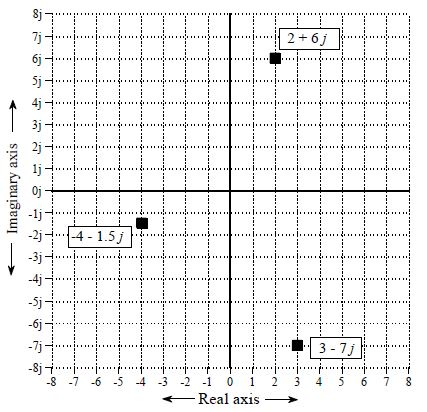
\includegraphics[scale=1]{complexPlane}  
			\caption[Contoh dari {\it complex plane} pada notasi {\it rectangular}]{Contoh dari {\it complex plane} pada notasi {\it rectangular}} 
			\label{fig:complexPlane} 
		\end{figure} 
	\item {\it Polar Notation}
		Pada notasi {\it Polar} terdapat {\it magnitude} / panjang vektor / {\it amplitude} dan {\it phase angle} yaitu besar sudut antara vektor dan sumbu positif $x$. Representasi {\it complex number} pada notasi {\it polar} seperti pada .
			\begin{equation}\label{eqn:complexNumberMag}
				M = \sqrt{(Re \:\: \mathsf{A})^2 + (Im \:\: \mathsf{A})^2}
			\end{equation}
			\begin{equation}\label{eqn:complexNumberPhase}
				\Theta = \arctan [\frac{Im \:\: \mathsf{A}}{Re \:\: \mathsf{A}}]
			\end{equation}
			
			\begin{figure} [H]
			\centering  
			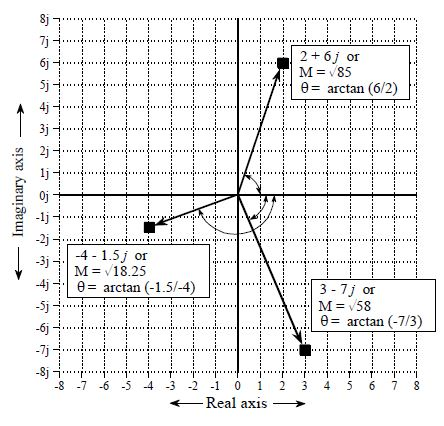
\includegraphics[scale=1]{complexPlanePolar}  
			\caption[Contoh dari {\it complex plane} pada notasi polar]{Contoh dari {\it complex plane} pada notasi polar} 
			\label{fig:complexPlanePolar} 
		\end{figure}
		Pada {\it complex number} terdapat {\it euler relation} dengan persamaan \ref{eqn:complexNumberEul}.
			\begin{equation}\label{eqn:complexNumberEul}
				e^{jx} = \cos (x) + j \sin (x)
			\end{equation}		
\end{itemize}

\subsection{Discrete Fourier Transform (DFT) \cite{pariyal:0:differentFFT} \cite{steven:0:dsp}}
\label{subsec:dft}

DFT dapat memiliki 2 versi yaitu {\it real version} dan {\it complex version} (\ref{sec:fourier}). DFT {\it complex version} dapat dikembangkan menjadi FFT (\ref{subsec:fft}). DFT yang menggunakan {\it complex number} memiliki persamaan seperti persamaan \ref{eqn:DFT}.
	\begin{equation}\label{eqn:DFT}
		X(k) =\sum_{n=0}^{N-1}x(n)\times e^{-j(\frac{2\pi}{N})nk} 
	\end{equation}
Pada persamaan \ref{eqn:DFT}, $N$ merupakan jumlah sample, $x(n)$ merupakan input dari sinyal pada domain waktu, dan $X(k)$ merupakan output dari sinyal pada domain frekuensi. 


\subsection{Fast Fourier Transform (FFT) \cite{pariyal:0:differentFFT} \cite{sidney:0:fft}}
\label{subsec:fft}
{\it Fast Fourier Transform} adalah teknik komputasi DFT yang lebih efisien. FFT hanya memiliki cara menghitung DFT yang lebih cepat. Hasil dari FFT memiliki sama dengan hasil dari DFT. Salah satu contoh dari algoritma FFT adalah {\it Cooley-Tukey Algorithm}. 

Algoritma {\it Cooley-Tukey} yang menggunakan panjang ($N$) berkelipatan 2 disebut dengan {\it Radix-2 Algorithm}. Pada algoritma ini ada 2 jenis proses disebut dengan {\it Decimation in Time} (DIT) dan {\it Decimation in Frequency}. Jika masukan adalah sinyal pada domain waktu, maka 
diproses dengan DIT dan jika masukan sinyal pada domain frekuensi, maka diproses dengan DIF. DIT akan mengubah sinyal dari domain waktu ke domain frekuensi dan DIF akan mengubah sinyal dari domain frekuensi ke domain waktu. Setiap masukan untuk proses DIT dan DIF harus dalam urutan {\it bit reverse} (\ref{tab:bitreverse}) agar keluaran dari DIT dan DIF dalam urutan yang sebenarnya. Algoritma dari Radix-2 DIT dapat dilihat pada \ref{alg:DIT} dan contoh visual dari DIT dengan panjang FFT adalah 8 pada Gambar~\ref{fig:DIT}.

\begin{algorithm}[htbp]
	\label{alg:DIT}
		\caption{Algoritma DIT}
		\begin{algorithmic}[1]
		\State \textbf{Input  :} masukan sinyal dalam domain waktu dan sudah dalam urutan {\it bit-reverse}
		\State \textbf{Output :} masukan sinyal dalam domain frekuensi	
			\For {Setiap kelipatan 2 dari panjang FFT ($N$)}
				\For{Setiap indeks semua masukan tiap bagian $N$}	
					\For {Setiap indeks ($k$) sampai $N/2$}
						\State  masukan dengan indeks genap ditambah dengan 
								masukan dengan indeks ganjil yang sudah dikalikan dengan $W^k_N$ 	
						\State masukan dengan indeks ganjil dikurang dengan
							   masukan dengan indeks ganjil yang sudah dikalikan dengan $W^k_N$
					\EndFor				
				\EndFor		
			\EndFor
			\State return finalOrder
	\end{algorithmic}
	\end{algorithm}

\begin{equation}\label{eqn:twiddle}
	W^k_N = e^{-j(\frac{2\pi k}{N})} 
\end{equation}

Persamaan \ref{eqn:twiddle} disebut juga dengan {\it twiddle factor}. Nilai $k$ pada persamaan ini adalah indeks bernilai sampai dengan $N/2$. 


\begin{table}[H]
	\label{tab:bitreverse}
	\centering
	\begin{tabular}{|c|c|c|c|}
	\hline	Index & Binary & Bit-reversed Binary & Bit-reversed Index\\
	\hline 0	& 000 & 000 & 0 \\
	\hline 1	& 001 & 100 & 4 \\
	\hline 2	& 010 & 010 & 2 \\
	\hline 3	& 011 & 110 & 6 \\
	\hline 4	& 100 & 001 & 1 \\
	\hline 5	& 101 & 101 & 5 \\
	\hline 6	& 110 & 011 & 3 \\
	\hline 7	& 111 & 111 & 7 \\
	\hline
	\end{tabular}
	\caption{Tabel contoh {\it bit reverse} dari indeks 0 sampai 7 }
\end{table}
\begin{figure} [H]
	\centering  
	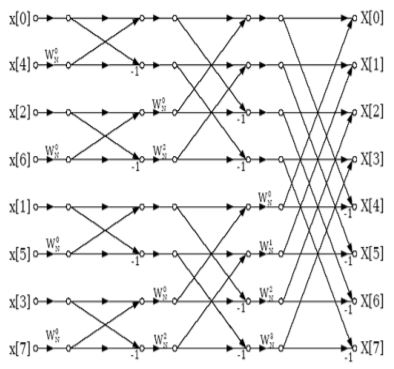
\includegraphics[scale=1]{DIT}  
	\caption[contoh visual {\it Decimation In Time} dengan panjang 8 ]{contoh visual {\it Decimation In Time} dengan panjang 8} 
	\label{fig:DIT} 
\end{figure} 

Jika pada proses DIT masukan dengan indeks genap dikurang dengan masukan indeks ganjil yang sudah dikalikan dengan $W^k_N$ dan masukan indeks ganjil ditambah dengan masukan dengan indeks ganjil yang sudah dikalikan dengan $W^k_N$, maka proses tersebut menjadi proses DIF.

Selain dari {\it Cooley-Tukey Algorithm} terdapat pula algoritma FFT lain seperti {\it Prime factor Algorithm}, {\it Rader's FFT Algorithm}, {\it Bluestein's FFT Algorithm}, dan {\it Winograd FFT Algorithm}.

\subsection{Short Time Fourier Transform (STFT) \cite{alan:0:dtsp}}
\label{subsec:stft}
%==========================================================
  
Algoritma ini adalah pengembangan dari algoritma FFT \cite{yani:0:stft}. Pada algoritma ini masukan sinyal pada domain waktu dicuplik selama waktu tertentu atau sebesar {\it window}. Setiap window dari cuplikan waktu ({\it segment}) dilakukan FFT untuk mendapatkan frekuensi pada waktu cuplikkan. Algoritma ini memiliki notasi sebagai berikut \cite{seo:0:stft}.
	\begin{equation}\label{eqn:STFT}
		S(\omega,\tau)=Fs(t) w(\tau - t) \\
	\end{equation}
	Keterangan : \\
	\begin{itemize}
		\item $S(\omega,\tau)$ = hasil dari STFT, $\omega$ adalah frekuensi dan $\tau$ adalah waktu. \\
		\item $s(t)$ = input sinyal \\
		\item $w(t)$ = fungsi window \\
		\item $F$ = Fourier Transform untuk input sinyal yang sudah menerapkan window
	\end{itemize}

	{\it Segment} dapat saling bertumpukkan ({\it overlap}). Kegunaan dari {\it windows function} adalah untuk meningkatkan hasil dari {\it fourier tranform}\cite{hp:10:hp}. {\it Windows function} akan memengaruhi hasil FFT bergantung pada jenis gelombang. Terdapat 4 jenis gelombang yang umum yaitu, {\it Sinus wave}, {\it Square wave}, {\it Transient wave}, dan {\it Impulse wave} (Gambar~\ref{fig:gelombang}). 
	\begin{figure} [H]
	\centering  
	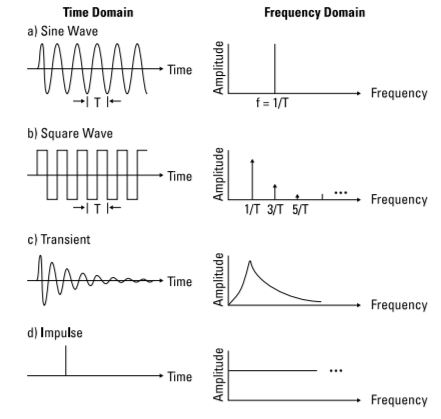
\includegraphics[scale=1]{gelombang}  
	\caption[Jenis gelombang]{{\it Jenis gelombang}} 
	\label{fig:gelombang} 
	\end{figure} 
	
	Pada gelombang {\it transient}, {\it window function} yang terbaik adalah {\it Rectangle Window} \cite{hp:10:hp}. Gelombang {\it trancient} bersifat {\it aperiodic} sehingga sinyal yang ditangkap tidak harus direduksi. Pada gelombang yang selain {\it trancient}, {\it windows function} dapat meningkatkan hasil pada {\it special measurement situations}. Berikut contoh - contoh dari {\it window function} \cite{yiwen:0:stft} :
	\begin{itemize}
		\item Rectangular Window :
			\begin{equation}\label{eqn:rectW}
				w_R[n]= 1 ,n = 0,1,2,..., N -1 \\
				w_R[n]= 0 , elsewhere
			\end{equation}
			Keterangan : \\
			\begin{itemize}
				\item $N$ = panjang window
			\end{itemize}
		\item Hanning window :
			\begin{equation}\label{eqn:hannW}
				w[n]= 0.5 (1.0 - cos(\frac{2n\pi}{N})) , n = 0, 1, 2, ... , N-1
			\end{equation}
			\begin{itemize}
				\item $N$ = panjang window
			\end{itemize}
		\item Hamming window :
			\begin{equation}\label{eqn:hammW}
				w[n]= 0.54 - 0.46cos[\frac{2n\pi}{N}] , n = 0, 1, 2, ... , N-1
			\end{equation}
			\begin{itemize}
				\item $N$ = panjang window
			\end{itemize}
	\end{itemize}

Hasil grafik dari {\it magnitude} STFT disebut dengan spectrogram. {\it Magnitude} didapatkan dari operasi {\it absolute} (\ref{eqn:complexNumberMag}) hasil dari STFT. Dari spectrogram terlihat perubahan besaran amplitudo dari frekuensi pada selang waktu. 
 Berikut contoh dari spectrogram (Gambar~\ref{fig:Spectrogramcth}).

\begin{figure} [H]
	\centering  
	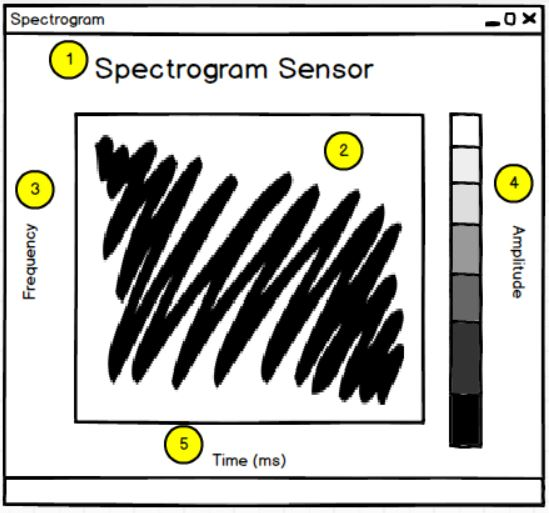
\includegraphics[scale=0.3]{Spectrogram}  
	\caption[Contoh Spectrogram]{Contoh Spectrogram} 
	\label{fig:Spectrogramcth} 
\end{figure}
\begin{itemize}
	\item Sumbu $x$ pada spectrogram adalah waktu
	\item Sumbu $y$ pada spectrogram adalah frekuensi
	\item Sumbu $z$ pada spectrogram adalah {\it amplitude / magnitude} hasil STFT
\end{itemize}

Dari Gambar~\ref{fig:Spectrogramcth} terlihat perubahan warna dari warna gelap ke warna terang. Perubahan warna ini menunjukan perubahan 
dari amplitudo frekuensi dari waktu ke waktu. Warna terterang pada spectrogram menunjukan frekuensi dominan dari sampel tersebut.
%==============================================================================
\section{PreonVM \& Preon32}
Preon32 adalah sensor node buatan VIRTENIO dan PreonVM merupakan {\it operating software} yang digunakan Preon32. Berikut penjelasan lebih
detil tentang PreonVM dan Preon32.

\subsection{PreonVM} 
PreonVM merupakan {\it virtual machine} buatan VIRTENIO untuk{\it embedded system} dengan sumber daya yang sangat kecil \footnote{https://www.virtenio.com/en/portfolio-items/preonvm/}. {\it Virtual machine} dari PreonVM sudah sangat optimal dan sudah berjalan langsung di {\it microcontroller}, sehingga tidak membutuhkan sistem operasi tambahan pada sensor node. {\it Developer} dapat menggunakan {\it libraries} yang disediakan PreonVM dalam bahasa pemrograman Java untuk mengambil data dari sensor dan mengatur aktuator pada sensor node.

\subsubsection{Fitur PreonVM}
PreonVM memiliki fitur sebagai berikut:
\begin{itemize}
	\item Aplikasi diprogram dengan bahasa pemrograman Java
	\item Mendukung semua tipe data pada Java ({\it char}, {\it byte}, {\it int}, {\it long}, {\it float} atau {\it double})
	\item Jumlah {\it thread} tidak dibatasi
	\item {\it Exception handling} ({\it try}, {\it catch}, {\it Exception}, atau {\it Runtime Exception})
	\item {\it Garbage collection} dengan {\it memory defragmentation}
	\item {\it System properties} untuk mengonfigurasi aplikasi
\end{itemize}

\subsubsection{Kelebihan PreonVM}
PreonVM menggunakan {\it object-oriented programming} pada {\it virtual machine}-nya untuk {\it embedded system}. PreonVM dioptimasi sedemikian rupa agar aplikasi dapat dijalankan 8-bit sampai 32-bit {\it microcontroller} dengan 8KB RAM dan 128KB Flash minimum. {\it Virtual machine} PreonVM memampukan aplikasi secara independen berjalan pada arsitektur yang digunakan. Dengan demikian arsitektur yang berbeda tidak memengaruhi aplikasi yang dijalankan (Gambar~\ref{fig:PreonVM}). {\it Virtual machine} PreonVM juga mampu memisahkan proses yang dilakukan {\it hardware} dan {\it software}. 

\begin{figure} [H]
	\centering  
	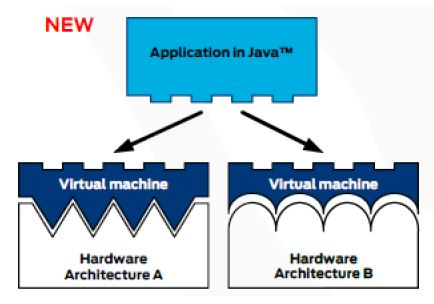
\includegraphics[scale=1]{PreonVM}  
	\caption[{\it Virtual machine} yang memampukan aplikasi berjalan secara independen]{{\it Virtual machine} yang memampukan aplikasi berjalan secara independen} 
	\label{fig:PreonVM} 
\end{figure} 

\subsubsection{Class Library PreonVM}
\label{subsubsec:library}
{\it Packages} yang terdapat pada PreonVM dapat dibagi menjadi 2 {\it package}, yaitu {\it package} dari Virtenio Tabel~\ref{tab:preonvm_virtenio_packages} dan {\it package} dari Java Tabel~\ref{tab:preonvm_java_packages}.
\begin{table}[H] %atau h saja untuk "kira kira di sini"
	\centering 
	\caption{Tabel Package dari Virtenio pada PreonVM}
	\label{tab:preonvm_virtenio_packages}
	\begin{tabular}{|p{8cm}|p{8cm}|}
	\hline
		Package & Deksripsi \\
    \hline
com.virtenio.crypt	 & Paket dari Virtenio untuk enkripsi dan dekripsi \\
com.virtenio.driver	 &\\
com.virtenio.driver.adc	 &\\
com.virtenio.driver.button	 &\\
com.virtenio.driver.can	 &\\
com.virtenio.driver.cpu	 &\\
com.virtenio.driver.device	 &\\
com.virtenio.driver.device.at86rf231	 &\\
com.virtenio.driver.flash	 &\\
com.virtenio.driver.gpio	 &\\
com.virtenio.driver.i2c	 &\\
com.virtenio.driver.irq	 & Paket dari Virtenio yang mengatur driver\\
com.virtenio.driver.led	 &\\
com.virtenio.driver.lin	 &\\
com.virtenio.driver.onewire	 &\\
com.virtenio.driver.pwm	 &\\
com.virtenio.driver.ram	 &\\
com.virtenio.driver.realtimeclock	 &\\
com.virtenio.driver.realtimecounter	 &\\
com.virtenio.driver.spi	 &\\
com.virtenio.driver.switch\_ &\\
com.virtenio.driver.timer	 &\\
com.virtenio.driver.usart	 &\\
com.virtenio.driver.watchdog	 &\\
\hline
\end{tabular}
\end{table}

\begin{table}[H] %atau h saja untuk "kira kira di sini"
	\centering 
	\caption{Tabel Package dari Virtenio pada PreonVM}
	\label{tab:preonvm_virtenio_packages1}
	\begin{tabular}{|p{8cm}|p{8cm}|}
	\hline
		Package & Deksripsi \\
    \hline
com.virtenio.flashlogger	&\\
com.virtenio.io	 &\\
com.virtenio.math &\\
com.virtenio.misc	 &\\
com.virtenio.net	& \\
com.virtenio.net.lowpan	 &\\
com.virtenio.preon32.cpu	  & Paket dari Virtenio untuk Flash, io, dan lainnya\\
com.virtenio.preon32.mainboard	 &\\
com.virtenio.preon32.node	& \\
com.virtenio.preon32.shuttle	& \\
com.virtenio.radio	& \\
com.virtenio.radio.ieee\_802\_15\_4	& \\
com.virtenio.route.aodv	 &\\
com.virtenio.vm.event	& \\
\hline
\end{tabular}
\end{table}

\begin{table}[H] %atau h saja untuk "kira kira di sini"
	\centering 
	\caption{Tabel Package dari Java pada PreonVM}
	\label{tab:preonvm_java_packages}
	\begin{tabular}{|p{8cm}|p{8cm}|}
	\hline
		Package & Deksripsi \\
    \hline
java.io	 &\\
java.lang	 &\\
java.lang.ref	 &\\
java.math	 &\\
java.nio	& \\
java.nio.channels	 & Paket dari Java\\
java.text	& \\
java.util	& \\
java.util.concurrent	& \\
java.util.concurrent.atomic	& \\
java.util.concurrent.locks	& \\
java.util.regex &\\
\hline
	\end{tabular}
	
\end{table}

\subsection{Preon32}  \footnote{https://www.virtenio.com/en/portfolio-items/preon32/}
Preon32 merupakan sensor node buatan Virtenio. PreonVM digunakan sebagai {\it operating software} untuk sensor node ini. Preon32 dapat menjadi 2 jenis yaitu Preon32 versi biasa dan Preon32 versi tambahan. Preon32 versi biasa memiliki sensor suhu ({\it temperature sensor}), sensor cahaya ({\it light intensity sensor}), sensor kelembaban udara ({\it relative humidity sensor}), sensor tekanan udara ({\it air pressure sensor / barometer}), dan sensor getaran ({\it acceleration sensor / accelerometer}). Pada Preon32 versi tambahan dilengkapi dengan sensor pendeteksi medan magnet dan {\it gyroscope} (Gambar~\ref{fig:Preon32}). 

Satuan pengukuran {\it raw data} dari sensor akselerometer di Preon32 adalah {\it bits}.  Hasil pengukuran ini dapat diubah menjadi satuan standar gravitasi  ($1g = 9.80665m/s^2$). \footnote{https://en.wikipedia.org/wiki/Standard\_gravity}

\begin{figure} [H]
	\centering  
	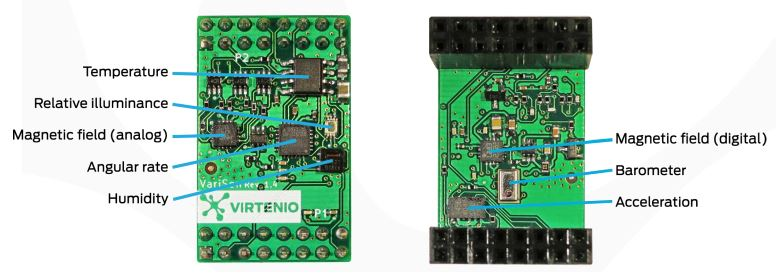
\includegraphics[scale=1]{Preon32}  
	\caption[Preon32]{Preon32} 
	\label{fig:Preon32} 
\end{figure} 

\subsubsection{Spesifikasi Sensor Preon32}
\label{subsubsec:specPreon32}
Berikut spesifikasi sensor yang dimiliki Preon32:
	\begin{itemize}
		\item sensor suhu ({\it temperature sensor})
			\begin{itemize}
    			\item Manufacture : Analog Devices
    			\item Model : ADT7410
    			\item Interface : digital, I2C
    			\item Resolution : 16-Bit
    			\item Range : -40$^{\circ}$C sampai +105$^{\circ}$C
    			\item Accuracy : $\pm$0.5$^{\circ}$C
			\end{itemize}
		\item sensor cahaya ({\it light intensity sensor})
			\begin{itemize}
				\item Manufacture : Rohm
    			\item Model : BH1715FVC
   				\item Interface : digital, I2C
    			\item Resolution : 16-Bit
    			\item Range : 1 lx to 65355 lx
			\end{itemize}
		\item sensor kelembaban udara ({\it relative humidity sensor})
			\begin{itemize}
    			\item Manufacture : Sensirion
    			\item Model : SHT21
    			\item Interface : digital, I2C
    			\item Resolution : 12-Bit
    			\item Range : 0 \%RH sampai 100 \%RH
    			\item Accuracy : $\pm$2,0 \%RH (typ.)
			\end{itemize}
		\item sensor tekanan udara ({\it air pressure sensor / barometer})
			\begin{itemize}
    			\item Manufacture : Freescale
    			\item Model : MPL115A2
    			\item Interface : digital, I2C
    			\item Resolution : 0,15 kPa
    			\item Range : 50 kPa sampai 115 kPa
    			\item Accuracy : $\pm$1.0 kPa
			\end{itemize}
		\item sensor getaran ({\it acceleration sensor / accelerometer}) 
			\begin{itemize}
    			\item Manufacture : Analog Devices
    			\item Model : ADXL345
    			\item Interface : digital, SPI
    			\item Resolution : 13 Bit per axis
    			\item Range : $\pm$16 g, 3 axis
    			\item Accuracy : 3,9 mg/LSB
			\end{itemize}
	\end{itemize}







